% !TeX program = xelatex
\documentclass[12pt,a4paper]{article}
\usepackage{fontspec}
\setmainfont{Times New Roman}[Path=C:/Windows/Fonts/,UprightFont=times.ttf,BoldFont=timesbd.ttf,ItalicFont=timesi.ttf,BoldItalicFont=timesbi.ttf]
\usepackage{amsmath,amssymb,amsfonts}
\usepackage[left=1.5cm,right=1.5cm,top=1.4cm,bottom=1.6cm,headheight=17pt]{geometry}
\usepackage{enumitem,array,graphicx,tikz,fancyhdr,needspace}
\usetikzlibrary{arrows.meta,calc,patterns}
% Sửa số đề và số trang đề thực tế sau khi biên dịch/tách PDF.
\newcommand{\soDe}{10}
\newcommand{\soTrangDe}{4}
\newcommand{\maDe}{\ifnum\soDe<1000 0\fi\ifnum\soDe<100 0\fi\ifnum\soDe<10 0\fi\soDe}
\pagestyle{fancy}
\fancyhf{}
\lhead{\small\textbf{ÔN TẬP GIỮA KÌ I}}
\rhead{\small\textit{Biên soạn: Dương Gia Bảo}}
\rfoot{\small Trang \thepage/\soTrangDe\ - Mã đề: \maDe}
\renewcommand{\headrulewidth}{0.4pt}
\fancypagestyle{answers}{\rfoot{\small Trang \thepage\ - Mã đề: \maDe}}
\fancypagestyle{firstpage}{\fancyhead{}\renewcommand{\headrulewidth}{0pt}}
\setlength{\parindent}{0pt}
\setlength{\parskip}{2.5pt}
\setlength{\emergencystretch}{1em}
\setlist[enumerate,1]{label=\textbf{Câu \arabic*:},leftmargin=*,itemsep=5pt,topsep=2pt}
\setlist[enumerate,2]{label=\alph*),leftmargin=*,itemsep=2pt,topsep=2pt}
\newcommand{\bonpa}[4]{\par\nobreak\smallskip\nobreak\noindent
\begin{tabular}{@{}p{0.47\linewidth}p{0.47\linewidth}@{}}
\textbf{A.} #1 & \textbf{B.} #2\\[8pt]
\textbf{C.} #3 & \textbf{D.} #4\end{tabular}}
\newcommand{\loigiai}[1]{\par\medskip\Needspace{4\baselineskip}\noindent\textbf{#1}\par\nobreak}
\newcommand{\otraloi}{\par\nobreak\smallskip\noindent\textit{Trả lời:}\quad\fbox{\rule{0pt}{11pt}\makebox[0.3cm]{}}\,\fbox{\rule{0pt}{11pt}\makebox[0.3cm]{}}\,\fbox{\rule{0pt}{11pt}\makebox[0.3cm]{}}\,\fbox{\rule{0pt}{11pt}\makebox[0.3cm]{}}}
\begin{document}
\thispagestyle{firstpage}
\noindent
\begin{minipage}[t]{0.35\textwidth}
    \centering
    {\fontsize{13}{15}\selectfont\textbf{ÔN TẬP GIỮA KÌ I}}\\[4pt]
    \textit{Biên soạn: Dương Gia Bảo}\\[5pt]
    \setlength{\fboxrule}{0.8pt}%
    \setlength{\fboxsep}{4pt}%
    \fbox{\begin{minipage}{0.83\linewidth}
        \centering
        {\fontsize{13}{15}\selectfont\textbf{ĐỀ ÔN TẬP}\\[2pt]\textbf{CHƯƠNG I VÀ II}}\\[4pt]
        \textit{(Đề thi gồm có \ifnum\soTrangDe<10 0\fi\soTrangDe\ trang)}
    \end{minipage}}
\end{minipage}\hfill
\begin{minipage}[t]{0.63\textwidth}
    \centering
    {\fontsize{13}{15}\selectfont\textbf{ÔN TẬP KIỂM TRA GIỮA KÌ I}\\[2pt]
    \textbf{NĂM HỌC 2026 - 2027}}\\[5pt]
    {\fontsize{14}{16}\selectfont\textbf{Môn: TOÁN - Lớp 12 (ĐỀ SỐ \soDe)}}\\[4pt]
    {\fontsize{11.5}{13}\selectfont\textit{Thời gian làm bài: 90 phút, không kể thời gian giao đề}}\\[5pt]
    \setlength{\fboxrule}{0.8pt}%
    \setlength{\fboxsep}{5pt}%
    \fbox{\makebox[3cm]{\fontsize{14}{16}\selectfont\textbf{Mã đề: \maDe}}}
\end{minipage}
\par\vspace{2pt}
\hrule height 0.6pt
\vspace{3pt}
\noindent\textit{Họ và tên học sinh:}\dotfill\hspace{1cm}\textit{Lớp:}\makebox[3.5cm]{\dotfill}
\par\vspace{2pt}
\hrule height 0.6pt
\vspace{3pt}

\section*{\large PHẦN I. Câu trắc nghiệm nhiều phương án lựa chọn}
\textit{Thí sinh trả lời từ câu 1 đến câu 12. Mỗi câu chỉ chọn một phương án.}
\begin{enumerate}
\item Cho hàm số $y=x^3-3x^2+1$. Hàm số đã cho nghịch biến trên khoảng nào dưới đây?
\bonpa{$(0;2)$.}{$(-\infty;0)$.}{$(2;+\infty)$.}{$(-1;1)$.}

\item Cho hàm số $y=-x^3+3x^2+9x-2$. Giá trị cực đại của hàm số đã cho bằng
\bonpa{$-7$.}{$25$.}{$3$.}{$-1$.}

\item Cho hàm số $f(x)=\dfrac{2x-1}{x+2}$. Giá trị lớn nhất của hàm số trên đoạn $[0;3]$ bằng
\bonpa{$-\dfrac{1}{2}$.}{$2$.}{$1$.}{$0$.}

\item Phương trình đường tiệm cận đứng của đồ thị hàm số $y=\dfrac{3x+1}{x-2}$ là
\bonpa{$y=3$.}{$x=-2$.}{$y=-2$.}{$x=2$.}

\item Đường tiệm cận xiên của đồ thị hàm số $y=\dfrac{x^2-3x+1}{x-2}$ có phương trình là
\bonpa{$y=x-1$.}{$y=x+1$.}{$y=x-3$.}{$y=2x-1$.}

\item Đường cong trong hình vẽ bên là đồ thị của hàm số nào dưới đây?
\par\nobreak\smallskip
\begin{minipage}[c]{0.62\linewidth}
\bonpa{$y=\dfrac{x^2-x+1}{x-1}$.}{$y=\dfrac{x^2-2x+2}{x-1}$.}{$y=\dfrac{x^2+2x+2}{x+1}$.}{$y=\dfrac{x^2+1}{x-1}$.}
\end{minipage}\hfill
\begin{minipage}[c]{0.36\linewidth}\centering
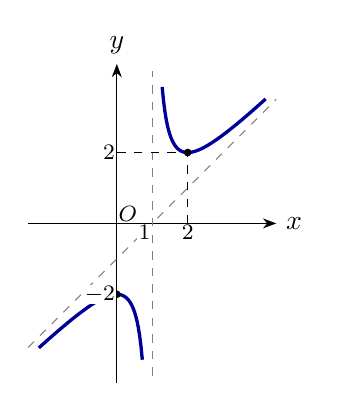
\begin{tikzpicture}[x=0.45cm,y=0.45cm,>=Stealth]
\draw[->] (-2.5,0)--(4.5,0) node[right] {$x$};
\draw[->] (0,-4.5)--(0,4.5) node[above] {$y$};
\draw[dashed,gray] (1,-4.3)--(1,4.3);
\draw[dashed,gray] (-2.5,-3.5)--(4.5,3.5);
\draw[very thick,blue!60!black,domain=-2.2:0.72,samples=80] plot (\x,{(\x*\x-2*\x+2)/(\x-1)});
\draw[very thick,blue!60!black,domain=1.28:4.2,samples=80] plot (\x,{(\x*\x-2*\x+2)/(\x-1)});
\draw[dashed] (2,0)--(2,2)--(0,2);
\fill (0,-2) circle (1.4pt);
\fill (2,2) circle (1.4pt);
\node[above right,fill=white,inner sep=0.5pt] at (0,0) {\footnotesize $O$};
\node[below left,fill=white,inner sep=0.5pt] at (1,0) {\footnotesize $1$};
\node[below,fill=white,inner sep=0.5pt] at (2,0) {\footnotesize $2$};
\node[left,fill=white,inner sep=0.5pt] at (0,-2) {\footnotesize $-2$};
\node[left,fill=white,inner sep=0.5pt] at (0,2) {\footnotesize $2$};
\end{tikzpicture}
\end{minipage}
\end{enumerate}

\newpage
\begin{enumerate}[start=7]
\item Khi nuôi cá thí nghiệm trong hồ, người ta nhận thấy nếu trên mỗi đơn vị diện tích mặt hồ thả $n$ con cá thì trung bình mỗi con cá sau một vụ thu hoạch cân nặng $P(n)=480-20n$ (gam) ($0<n<24$). Tổng khối lượng cá thu hoạch được trên một đơn vị diện tích sau một vụ là $f(n)=n\cdot P(n)=480n-20n^2$ (gam). Hỏi cần thả bao nhiêu con cá trên mỗi đơn vị diện tích để sau một vụ thu hoạch tổng khối lượng cá đạt giá trị lớn nhất?
\bonpa{$14$.}{$10$.}{$12$.}{$16$.}

\item Cho hình hộp chữ nhật $ABCD.A'B'C'D'$. Vectơ nào dưới đây bằng tổng ba vectơ $\vec{AB}+\vec{AD}+\vec{AA'}$?
\bonpa{$\vec{AC}$.}{$\vec{BD'}$.}{$\vec{A'C}$.}{$\vec{AC'}$.}

\item Trong không gian $Oxyz$, cho điểm $A(2;-3;5)$. Tọa độ hình chiếu vuông góc của điểm $A$ lên mặt phẳng $(Oxy)$ là
\bonpa{$(2;-3;0)$.}{$(0;0;5)$.}{$(2;0;5)$.}{$(0;-3;5)$.}

\item Trong không gian $Oxyz$, cho hai vectơ $\vec{a}=(1;-2;3)$ và $\vec{b}=(2;1;-1)$. Tọa độ của vectơ $\vec{u}=2\vec{a}+3\vec{b}$ là
\bonpa{$(4;-1;2)$.}{$(8;-1;3)$.}{$(8;-7;9)$.}{$(5;0;2)$.}

\item Trong không gian $Oxyz$, cho hai vectơ $\vec{u}=(2;1;-2)$ và $\vec{v}=(-3;4;1)$. Tích vô hướng $\vec{u}\cdot\vec{v}$ bằng
\bonpa{$4$.}{$-2$.}{$-4$.}{$6$.}

\item Trong không gian $Oxyz$, cho hai điểm $A(1;-1;2)$ và $B(3;1;3)$. Độ dài đoạn thẳng $AB$ bằng
\bonpa{$\sqrt{5}$.}{$9$.}{$\sqrt{7}$.}{$3$.}
\end{enumerate}

\vspace{3pt}
\section*{\large PHẦN II. Câu trắc nghiệm đúng hoặc sai}
\textit{Thí sinh trả lời từ câu 1 đến câu 4. Trong mỗi ý a), b), c), d) ở mỗi câu, thí sinh chọn đúng hoặc sai.}
\begin{enumerate}
\item Cho hàm số $y=f(x)=\dfrac{x^2-3x+6}{x-1}$.
\begin{enumerate}
\item Tập xác định của hàm số là $D=\mathbb{R}\setminus\{1\}$.
\item Đạo hàm của hàm số là $f'(x)=\dfrac{x^2-2x-3}{(x-1)^2}$.
\item Đồ thị hàm số có đường tiệm cận xiên là đường thẳng $y=x-2$.
\item Khoảng cách giữa hai điểm cực trị của đồ thị hàm số bằng $6\sqrt{2}$.
\end{enumerate}
\end{enumerate}

\newpage
\begin{enumerate}[start=2]
\item Một xưởng may công nghiệp sản xuất áo khoác xuất khẩu với số lượng $x$ nghìn chiếc mỗi tháng ($0 < x \le 40$). Chi phí sản xuất (tính bằng triệu đồng) được cho bởi hàm số $C(x)=x^3-25x^2+400x+800$. Doanh thu từ việc bán áo khoác (tính bằng triệu đồng) được cho bởi hàm số $R(x)=1000x-10x^2$. Lợi nhuận của xưởng may là $P(x)=R(x)-C(x)$.
\begin{enumerate}
\item Chi phí cố định của xưởng may khi chưa sản xuất áo khoác nào là $800$ triệu đồng.
\item Doanh thu của xưởng may khi bán được $20$ nghìn chiếc áo khoác là $16000$ triệu đồng.
\item Hàm lợi nhuận của xưởng may theo số lượng $x$ là $P(x)=-x^3+15x^2+600x-800$.
\item Xưởng may đạt lợi nhuận lớn nhất trong tháng khi sản xuất $25$ nghìn chiếc áo khoác.
\end{enumerate}

\item Trong không gian $Oxyz$, cho ba điểm $A(2;1;0)$, $B(4;2;2)$ và $C(1;3;0)$.
\begin{enumerate}
\item Tọa độ của vectơ $\vec{AB}$ là $\vec{AB}=(2;1;2)$.
\item Trọng tâm $G$ của tam giác $ABC$ có tọa độ là $G\left(\dfrac{7}{3};2;\dfrac{2}{3}\right)$.
\item Tích vô hướng $\vec{AB}\cdot\vec{AC}=0$, suy ra tam giác $ABC$ là tam giác vuông tại $A$.
\item Tọa độ điểm $D$ để tứ giác $ABCD$ là hình bình hành là $D(1;2;0)$.
\end{enumerate}

\item Một vật trang trí nghệ thuật có trọng lượng $P=240\text{ N}$ được treo cân bằng vào trần nhà nằm ngang bằng ba sợi dây cáp mảnh không dãn có chiều dài bằng nhau. Ba đầu dây trên trần nhà được cố định tại ba điểm $A, B, C$ tạo thành một tam giác đều, đầu còn lại của ba sợi dây được buộc chung vào vật tại điểm $O$. Chọn hệ trục toạ độ $Oxyz$ có gốc tại $O$, trục $Oz$ hướng thẳng đứng lên trần nhà (ngược hướng trọng lực). Khi đó trọng lực tác dụng lên vật là $\vec{P}=(0;0;-240)$ (đơn vị: N). Lực căng của ba sợi dây tác dụng lên móc treo $O$ lần lượt là $\vec{F}_1, \vec{F}_2, \vec{F}_3$. Biết ba lực này có cùng độ lớn $|\vec{F}_1|=|\vec{F}_2|=|\vec{F}_3|=F$, cùng tạo với phương thẳng đứng (trục $Oz$) một góc $60^\circ$, và hình chiếu của chúng lên mặt phẳng $(Oxy)$ đôi một tạo với nhau một góc $120^\circ$.
\begin{enumerate}
\item Do vật ở trạng thái cân bằng nên ta có hệ thức $\vec{F}_1+\vec{F}_2+\vec{F}_3+\vec{P}=\vec{0}$.
\item Hợp lực của ba lực căng dây $\vec{F}=\vec{F}_1+\vec{F}_2+\vec{F}_3$ có độ lớn bằng $240\text{ N}$ và cùng hướng với vectơ đơn vị $\vec{k}$ của trục $Oz$.
\item Độ lớn của mỗi lực căng dây là $F=160\text{ N}$.
\item Góc tạo bởi mỗi sợi dây cáp và mặt phẳng nằm ngang của trần nhà bằng $60^\circ$.
\end{enumerate}
\end{enumerate}

\vspace{3pt}
\section*{\large PHẦN III. Câu trắc nghiệm trả lời ngắn}
\textit{Thí sinh trả lời từ câu 1 đến câu 6. Mỗi câu trả lời đúng thí sinh được 0,5 điểm.}
\begin{enumerate}
\item Tìm số giá trị nguyên của tham số $m\in[-10;10]$ để hàm số $y=\dfrac{1}{3}x^3-mx^2+(m+6)x-2027$ đồng biến trên khoảng $(-\infty;+\infty)$.
\otraloi

\item Trong không gian $Oxyz$, cho hình hộp $ABCD.A'B'C'D'$ có tọa độ các đỉnh $A(1;1;1)$, $B(3;2;1)$, $D(2;4;2)$ và $A'(2;1;5)$. Tìm tọa độ đỉnh $C'(x;y;z)$, sau đó tính tổng $S=x+y+z$.
\otraloi
\end{enumerate}

\newpage
\begin{enumerate}[start=3]
\item Cho hàm số $y=\dfrac{x^2+mx+4}{x-2}$ ($m$ là tham số thực). Có bao nhiêu giá trị nguyên của tham số $m\in[-10;10]$ để đồ thị hàm số có hai điểm cực trị nằm về hai phía của trục tung?
\otraloi

\item Một người đứng ở mặt đất điều khiển hai flycam: Flycam I ở vị trí $A$ cách vị trí điều khiển $150\text{ m}$ về phía nam, $200\text{ m}$ về phía đông và cách mặt đất $50\text{ m}$. Flycam II ở vị trí $B$ cách vị trí điều khiển $180\text{ m}$ về phía bắc, $240\text{ m}$ về phía tây và cách mặt đất $60\text{ m}$. Chọn hệ trục toạ độ $Oxyz$ với gốc $O$ tại vị trí người điều khiển trên mặt đất, trục $Ox$ hướng nam, trục $Oy$ hướng đông, trục $Oz$ thẳng đứng hướng lên bầu trời (đơn vị trên mỗi trục tính theo mét). Khoảng cách giữa hai flycam bằng bao nhiêu mét (làm tròn kết quả đến hàng đơn vị)?
\otraloi

\item Người ta muốn làm một chiếc bể chứa nước bằng tôn không nắp dạng hình hộp chữ nhật có thể tích bằng $36\text{ m}^3$. Đáy bể là hình chữ nhật có chiều dài gấp đôi chiều rộng. Gọi chiều rộng của đáy bể là $x\text{ m}$, chiều cao của bể là $h\text{ m}$ (hình vẽ minh họa). Để tiết kiệm vật liệu nhất, diện tích toàn phần (không nắp) của bể phải đạt giá trị nhỏ nhất. Hỏi diện tích toàn phần nhỏ nhất của bể bằng bao nhiêu mét vuông?
\begin{center}
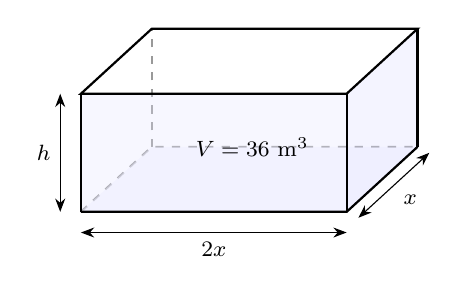
\begin{tikzpicture}[x=0.75cm,y=0.75cm,>=Stealth]
\coordinate (A) at (0,0);
\coordinate (B) at (4.5,0);
\coordinate (C) at (5.7,1.1);
\coordinate (D) at (1.2,1.1);
\coordinate (A1) at (0,2.0);
\coordinate (B1) at (4.5,2.0);
\coordinate (C1) at (5.7,3.1);
\coordinate (D1) at (1.2,3.1);

\draw[dashed,thick,gray!80] (A)--(D)--(C);
\draw[dashed,thick,gray!80] (D)--(D1);

\fill[blue!5,opacity=0.5] (A)--(B)--(C)--(D)--cycle;
\fill[blue!10,opacity=0.3] (A)--(B)--(B1)--(A1)--cycle;
\fill[blue!15,opacity=0.3] (B)--(C)--(C1)--(B1)--cycle;

\draw[thick] (A)--(B)--(C);
\draw[thick] (A1)--(B1)--(C1)--(D1)--cycle;
\draw[thick] (A)--(A1) (B)--(B1) (C)--(C1);

\draw[<->] (0,-0.35)--(4.5,-0.35) node[midway,below] {\footnotesize $2x$};
\draw[<->] (4.7,-0.1)--(5.9,1.0) node[midway,below right] {\footnotesize $x$};
\draw[<->] (-0.35,0)--(-0.35,2.0) node[midway,left] {\footnotesize $h$};

\node at (2.9,1.1) {\footnotesize $V = 36\text{ m}^3$};
\end{tikzpicture}
\par\vspace{1pt}{\footnotesize\textit{Hình minh họa bể chứa nước không nắp.}}
\end{center}
\otraloi

\item Một giàn khoan dầu $S$ cách bờ biển thẳng một khoảng $SH=6\text{ km}$ ($H$ là hình chiếu vuông góc của $S$ lên bờ biển). Nhà máy lọc dầu $N$ nằm trên bờ biển cách điểm $H$ một khoảng $HN=15\text{ km}$. Người ta dự định đặt đường ống dẫn dầu gồm hai đoạn: đoạn ống ngầm dưới biển nối từ giàn khoan $S$ đến một vị trí $C$ trên bờ biển (với $C$ nằm giữa $H$ và $N$), và đoạn ống trên đất liền nối từ $C$ đến nhà máy lọc dầu $N$ dọc theo bờ biển (hình vẽ minh họa). Biết chi phí lắp đặt mỗi kilômét ống ngầm dưới biển là $50$ triệu đồng, chi phí lắp đặt mỗi kilômét ống trên đất liền là $30$ triệu đồng. Tổng chi phí lắp đặt nhỏ nhất của toàn bộ đường ống dẫn dầu bằng bao nhiêu triệu đồng?
\begin{center}
\begin{tikzpicture}[x=0.65cm,y=0.65cm,>=Stealth]
\draw[thick,blue!50!gray] (-0.5,0)--(15.5,0) node[above,black] {\footnotesize Đường bờ biển};
\fill[cyan!10] (-0.5,-2.8) rectangle (15.5,0);
\node at (7.0,-1.9) {\textit{\footnotesize Biển}};
\node at (7.0,0.7) {\textit{\footnotesize Đất liền}};

\coordinate (H) at (0.5,0);
\coordinate (C) at (5.0,0);
\coordinate (N) at (15.0,0);
\coordinate (S) at (0.5,-2.5);

\fill (H) circle (2pt) node[above] {$H$};
\fill (C) circle (2pt) node[above] {$C$};
\fill (N) circle (2pt) node[above] {$N$};
\fill (S) circle (2pt) node[below] {$S$ (Giàn khoan)};

\draw[dashed] (S)--(H);
\draw (0.5,-0.3)--(0.8,-0.3)--(0.8,0);
\draw[line width=1.4pt,red!80!black] (S)--(C) node[midway,below right] {\footnotesize Ống ngầm dưới biển};
\draw[line width=1.5pt,orange!80!black] (C)--(N) node[midway,above] {\footnotesize Ống trên đất liền};

\draw[<->] (0.5,0.4)--(15.0,0.4) node[midway,above] {\footnotesize $15\text{ km}$};
\draw[<->] (-0.2,0)--(-0.2,-2.5) node[midway,left] {\footnotesize $6\text{ km}$};
\draw[<->] (0.5,-0.3)--(5.0,-0.3) node[midway,below] {\footnotesize $x$};
\end{tikzpicture}
\par\vspace{1pt}{\footnotesize\textit{Sơ đồ phương án lắp đặt đường ống dẫn dầu.}}
\end{center}
\otraloi
\end{enumerate}
\begin{center}\textbf{---------------- HẾT ----------------}\end{center}

\newpage\pagestyle{answers}
\begin{center}\Large\textbf{BẢNG ĐÁP ÁN TỔNG HỢP}\end{center}
\textbf{Phần I. Trắc nghiệm nhiều phương án lựa chọn}
\begin{center}
\renewcommand{\arraystretch}{1.5}
\begin{tabular}{|c|*{12}{c|}}\hline
Câu & 1&2&3&4&5&6&7&8&9&10&11&12\\\hline
Đáp án & A & B & C & D & A & B & C & D & A & B & C & D \\\hline
\end{tabular}
\end{center}

\textbf{Phần II. Đúng hoặc sai}
\begin{center}
\renewcommand{\arraystretch}{1.4}
\begin{tabular}{|c|c|c|c|c|}\hline
Câu & a) & b) & c) & d)\\\hline
1 & Đ & Đ & Đ & S\\\hline
2 & Đ & Đ & Đ & S\\\hline
3 & Đ & Đ & Đ & S\\\hline
4 & Đ & Đ & Đ & S\\\hline
\end{tabular}
\end{center}

\textbf{Phần III. Trả lời ngắn}
\begin{center}
\renewcommand{\arraystretch}{1.5}
\begin{tabular}{|c|c|c|c|c|c|c|}\hline
Câu & 1 & 2 & 3 & 4 & 5 & 6\\\hline
Đáp án & 6 & 16 & 12 & 550 & 54 & 690 \\\hline
\end{tabular}
\end{center}

\vspace{0.5cm}
\begin{center}
\large\textbf{HƯỚNG DẪN GIẢI CHI TIẾT}
\end{center}

\section*{PHẦN I}

\loigiai{Câu 1. Chọn A.}
Hàm số đã cho là $y=x^3-3x^2+1$.
Tập xác định: $D=\mathbb{R}$.
Đạo hàm: $y'=3x^2-6x=3x(x-2)$.
Ta có $y'<0 \iff 0 < x < 2$.
Do đó, hàm số nghịch biến trên khoảng $(0;2)$.

\loigiai{Câu 2. Chọn B.}
Hàm số đã cho là $y=-x^3+3x^2+9x-2$.
Tập xác định: $D=\mathbb{R}$.
Đạo hàm: $y'=-3x^2+6x+9=-3(x^2-2x-3)=-3(x-3)(x+1)$.
$y'=0 \iff x=3$ hoặc $x=-1$.
Đạo hàm cấp hai: $y''=-6x+6$.
Tại $x=3$: $y''(3)=-6(3)+6=-12<0 \implies x=3$ là điểm cực đại của hàm số.
Giá trị cực đại tương ứng là $y(3)=-(3)^3+3(3)^2+9(3)-2=-27+27+27-2=25$.

\loigiai{Câu 3. Chọn C.}
Hàm số $f(x)=\dfrac{2x-1}{x+2}$ xác định và liên tục trên đoạn $[0;3]$.
Đạo hàm: $f'(x)=\dfrac{2(x+2)-(2x-1)}{(x+2)^2}=\dfrac{5}{(x+2)^2}>0,\ \forall x\in[0;3]$.
Do hàm số luôn đồng biến trên đoạn $[0;3]$ nên giá trị lớn nhất đạt được tại điểm mút bên phải:
$\max_{[0;3]} f(x) = f(3) = \dfrac{2(3)-1}{3+2} = \dfrac{5}{5} = 1$.

\loigiai{Câu 4. Chọn D.}
Hàm số $y=\dfrac{3x+1}{x-2}$.
Tập xác định: $D=\mathbb{R}\setminus\{2\}$.
Vì $\lim_{x\to 2^+} \dfrac{3x+1}{x-2}=+\infty$ và $\lim_{x\to 2^-} \dfrac{3x+1}{x-2}=-\infty$ nên đường thẳng $x=2$ là đường tiệm cận đứng của đồ thị hàm số.

\loigiai{Câu 5. Chọn A.}
Hàm số $y=\dfrac{x^2-3x+1}{x-2}$.
Thực hiện phép chia đa thức tử cho mẫu:
$x^2-3x+1 = (x-1)(x-2) - 1 \implies y = x-1 - \dfrac{1}{x-2}$.
Vì $\lim_{x\to \pm\infty} [y - (x-1)] = \lim_{x\to \pm\infty} \left(-\dfrac{1}{x-2}\right) = 0$ nên đường tiệm cận xiên của đồ thị hàm số là đường thẳng $y=x-1$.

\loigiai{Câu 6. Chọn B.}
Quan sát đồ thị hàm số trong hình vẽ:
- Đường tiệm cận đứng là $x=1$, suy ra mẫu số triệt tiêu tại $x=1$ (loại đáp án C có mẫu $x+1$).
- Đường tiệm cận xiên đi qua điểm $(0;-1)$ và $(1;0)$, có phương trình $y=x-1$.
- Đồ thị cắt trục tung tại điểm $(0;-2)$. Kiểm tra các phương án:
  + Với $y=\dfrac{x^2-2x+2}{x-1}$: tại $x=0 \implies y=\dfrac{2}{-1}=-2$ (thỏa mãn).
  + Với $y=\dfrac{x^2-x+1}{x-1}$: tại $x=0 \implies y=\dfrac{1}{-1}=-1$ (không thỏa mãn).
- Đồ thị có điểm cực tiểu tại $(2;2)$ và cực đại tại $(0;-2)$.
Do đó, đồ thị đã cho là của hàm số $y=\dfrac{x^2-2x+2}{x-1}$.

\loigiai{Câu 7. Chọn C.}
Tổng khối lượng cá thu hoạch được trên một đơn vị diện tích là
$f(n)=480n-20n^2$ với $n\in(0;24)$.
Đạo hàm: $f'(n)=480-40n$.
Cho $f'(n)=0 \iff 480-40n=0 \iff n=12$.
Vì $f''(n)=-40<0$ nên hàm số $f(n)$ đạt giá trị lớn nhất tại $n=12$.
Vậy cần thả $12$ con cá trên mỗi đơn vị diện tích mặt hồ.

\loigiai{Câu 8. Chọn D.}
Trong hình hộp chữ nhật $ABCD.A'B'C'D'$, theo quy tắc hình bình hành cho đáy $ABCD$:
$\vec{AB}+\vec{AD}=\vec{AC}$.
Khi đó: $\vec{AB}+\vec{AD}+\vec{AA'} = \vec{AC}+\vec{AA'}$.
Xét hình bình hành $ACC'A'$, ta có $\vec{AC}+\vec{AA'}=\vec{AC'}$.
Vậy $\vec{AB}+\vec{AD}+\vec{AA'}=\vec{AC'}$ (quy tắc hình hộp).

\loigiai{Câu 9. Chọn A.}
Trong không gian $Oxyz$, hình chiếu vuông góc của điểm $A(x;y;z)$ lên mặt phẳng tọa độ $(Oxy)$ có tọa độ là $(x;y;0)$.
Với điểm $A(2;-3;5)$, hình chiếu vuông góc lên $(Oxy)$ là $(2;-3;0)$.

\loigiai{Câu 10. Chọn B.}
Ta có $\vec{a}=(1;-2;3) \implies 2\vec{a}=(2;-4;6)$.
$\vec{b}=(2;1;-1) \implies 3\vec{b}=(6;3;-3)$.
Suy ra $\vec{u}=2\vec{a}+3\vec{b}=(2+6;-4+3;6-3)=(8;-1;3)$.

\loigiai{Câu 11. Chọn C.}
Áp dụng biểu thức tọa độ của tích vô hướng:
$\vec{u}\cdot\vec{v} = u_x v_x + u_y v_y + u_z v_z = 2(-3) + 1(4) + (-2)(1) = -6 + 4 - 2 = -4$.

\loigiai{Câu 12. Chọn D.}
Khoảng cách giữa hai điểm $A(1;-1;2)$ và $B(3;1;3)$ là
$AB=\sqrt{(3-1)^2 + (1-(-1))^2 + (3-2)^2} = \sqrt{2^2+2^2+1^2} = \sqrt{4+4+1} = \sqrt{9}=3$.

\section*{PHẦN II}

\loigiai{Câu 1.}
Cho hàm số $y=f(x)=\dfrac{x^2-3x+6}{x-1}$.
\begin{enumerate}
\item Đúng: Biểu thức xác định khi và chỉ khi mẫu số khác 0: $x-1\ne 0 \iff x\ne 1$. Vậy $D=\mathbb{R}\setminus\{1\}$.
\item Đúng: Áp dụng công thức đạo hàm hàm phân thức:
$$f'(x)=\dfrac{(2x-3)(x-1)-(x^2-3x+6)\cdot 1}{(x-1)^2}=\dfrac{2x^2-5x+3-(x^2-3x+6)}{(x-1)^2}=\dfrac{x^2-2x-3}{(x-1)^2}.$$
\item Đúng: Thực hiện phép chia đa thức:
$x^2-3x+6 = (x-2)(x-1) + 4 \implies f(x) = x-2 + \dfrac{4}{x-1}$.
Do $\lim_{x\to \pm\infty} [f(x)-(x-2)] = \lim_{x\to \pm\infty}\dfrac{4}{x-1}=0$ nên đường thẳng $y=x-2$ là đường tiệm cận xiên của đồ thị hàm số.
\item Sai: Ta có $f'(x)=0 \iff x^2-2x-3=0 \iff x=-1$ hoặc $x=3$.
Với $x=-1 \implies y=\dfrac{1+3+6}{-2}=-5$, ta có điểm cực trị $A(-1;-5)$.
Với $x=3 \implies y=\dfrac{9-9+6}{2}=3$, ta có điểm cực trị $B(3;3)$.
Khoảng cách giữa hai điểm cực trị là
$$AB = \sqrt{(3-(-1))^2 + (3-(-5))^2} = \sqrt{4^2+8^2} = \sqrt{16+64} = \sqrt{80} = 4\sqrt{5} \ne 6\sqrt{2}.$$
\end{enumerate}

\loigiai{Câu 2.}
Hàm chi phí $C(x)=x^3-25x^2+400x+800$, hàm doanh thu $R(x)=1000x-10x^2$ ($0<x\le 40$).
\begin{enumerate}
\item Đúng: Chi phí cố định ban đầu ứng với số lượng sản phẩm $x=0$:
$C(0) = 0 - 0 + 0 + 800 = 800$ (triệu đồng).
\item Đúng: Doanh thu khi bán $20$ nghìn chiếc áo khoác:
$R(20) = 1000(20) - 10(20)^2 = 20000 - 4000 = 16000$ (triệu đồng).
\item Đúng: Hàm lợi nhuận của xưởng may:
$$P(x)=R(x)-C(x)=(1000x-10x^2)-(x^3-25x^2+400x+800)=-x^3+15x^2+600x-800.$$
\item Sai: Xét hàm lợi nhuận trên $(0;40]$:
$P'(x)=-3x^2+30x+600$.
$P'(x)=0 \iff -3(x^2-10x-200)=0 \iff -3(x-20)(x+10)=0 \iff x=20$ (do $x>0$).
Bảng biến thiên: $P'(x)>0$ trên $(0;20)$ và $P'(x)<0$ trên $(20;40)$.
Do đó, hàm số đạt cực đại tại $x=20$. Lợi nhuận lớn nhất đạt được khi sản xuất $20$ nghìn chiếc áo khoác (không phải $25$ nghìn chiếc).
\end{enumerate}

\loigiai{Câu 3.}
Trong không gian $Oxyz$, cho $A(2;1;0)$, $B(4;2;2)$, $C(1;3;0)$.
\begin{enumerate}
\item Đúng: Vectơ $\vec{AB}=(4-2;2-1;2-0)=(2;1;2)$.
\item Đúng: Tọa độ trọng tâm $G$ của tam giác $ABC$:
$$x_G=\dfrac{2+4+1}{3}=\dfrac{7}{3};\quad y_G=\dfrac{1+2+3}{3}=2;\quad z_G=\dfrac{0+2+0}{3}=\dfrac{2}{3} \implies G\left(\dfrac{7}{3};2;\dfrac{2}{3}\right).$$
\item Đúng: Ta có $\vec{AC}=(1-2;3-1;0-0)=(-1;2;0)$.
Tích vô hướng $\vec{AB}\cdot\vec{AC} = 2(-1) + 1(2) + 2(0) = -2 + 2 + 0 = 0$.
Suy ra $\vec{AB}\perp\vec{AC}$, hay tam giác $ABC$ vuông tại $A$.
\item Sai: Tứ giác $ABCD$ là hình bình hành khi và chỉ khi $\vec{AD}=\vec{BC}$.
Ta có $\vec{BC}=(1-4;3-2;0-2)=(-3;1;-2)$.
Gọi $D(x_D;y_D;z_D)$, khi đó $\vec{AD}=(x_D-2;y_D-1;z_D-0)$.
$$\begin{cases} x_D-2=-3\\ y_D-1=1\\ z_D-0=-2 \end{cases} \iff \begin{cases} x_D=-1\\ y_D=2\\ z_D=-2 \end{cases} \implies D(-1;2;-2) \ne (1;2;0).$$
\end{enumerate}

\loigiai{Câu 4.}
Vật trang trí có trọng lượng $P=240\text{ N}$ ở trạng thái cân bằng.
\begin{enumerate}
\item Đúng: Theo định luật cân bằng lực tĩnh học, tổng tất cả các lực tác dụng lên vật tại móc treo $O$ bằng vectơ không: $\vec{F}_1+\vec{F}_2+\vec{F}_3+\vec{P}=\vec{0}$.
\item Đúng: Từ hệ thức cân bằng, ta có $\vec{F}=\vec{F}_1+\vec{F}_2+\vec{F}_3=-\vec{P}$.
Vì trọng lực $\vec{P}=(0;0;-240)$ hướng thẳng đứng xuống dưới theo chiều âm của trục $Oz$, nên hợp lực $\vec{F}=(0;0;240)$ có phương thẳng đứng hướng lên, cùng hướng với vectơ đơn vị $\vec{k}=(0;0;1)$ của trục $Oz$ và có độ lớn $|\vec{F}|=240\text{ N}$.
\item Đúng: Do tính đối xứng đều của hệ ba dây cáp, góc giữa mỗi lực căng và trục $Oz$ là $\alpha=60^\circ$. Hình chiếu của ba lực lên mặt phẳng nằm ngang $(Oxy)$ có độ lớn bằng nhau và triệt tiêu nhau từng đôi một (hợp nhau góc $120^\circ$).
Chiếu phương trình lên trục $Oz$ thẳng đứng:
$$\begin{aligned}
F_{1z}+F_{2z}+F_{3z}-P=0 &\iff 3\cdot F\cos 60^\circ = P \iff 3\cdot F\cdot \dfrac{1}{2} = 240\\
&\iff 1{,}5F=240 \iff F=160\text{ N}.
\end{aligned}$$
\item Sai: Vì mỗi sợi dây cáp tạo với phương thẳng đứng (trục $Oz$) một góc $60^\circ$ và phương thẳng đứng vuông góc với mặt phẳng nằm ngang trần nhà ($90^\circ$), nên góc giữa sợi dây cáp và mặt phẳng nằm ngang của trần nhà là:
$$\beta = 90^\circ - 60^\circ = 30^\circ \ne 60^\circ.$$
\end{enumerate}

\section*{PHẦN III}

\loigiai{Câu 1.}
Hàm số đã cho là $y=\dfrac{1}{3}x^3-mx^2+(m+6)x-2027$.
Tập xác định: $D=\mathbb{R}$.
Đạo hàm: $y'=x^2-2mx+m+6$.
Hàm số đồng biến trên khoảng $(-\infty;+\infty)$ khi và chỉ khi
$y'\ge 0,\ \forall x\in\mathbb{R} \iff x^2-2mx+m+6\ge 0,\ \forall x\in\mathbb{R}$.
Vì hệ số của $x^2$ là $a=1>0$, tam thức bậc hai không âm với mọi $x\in\mathbb{R}$ khi và chỉ khi
$$\Delta' \le 0 \iff (-m)^2 - 1(m+6) \le 0 \iff m^2-m-6\le 0 \iff (m-3)(m+2)\le 0 \iff -2\le m\le 3.$$
Do $m\in[-10;10]$ và $m\in\mathbb{Z}$ nên $m\in\{-2;-1;0;1;2;3\}$.
Có tất cả $3-(-2)+1=6$ giá trị nguyên thỏa mãn.

\loigiai{Câu 2.}
Trong không gian $Oxyz$, cho hình hộp $ABCD.A'B'C'D'$ với $A(1;1;1)$, $B(3;2;1)$, $D(2;4;2)$, $A'(2;1;5)$.
Áp dụng quy tắc hình hộp cho đường chéo xuất phát từ đỉnh $A$:
$$\vec{AC'} = \vec{AB} + \vec{AD} + \vec{AA'}.$$
Ta tính các vectơ thành phần:
$\vec{AB} = (3-1; 2-1; 1-1) = (2; 1; 0)$.
$\vec{AD} = (2-1; 4-1; 2-1) = (1; 3; 1)$.
$\vec{AA'} = (2-1; 1-1; 5-1) = (1; 0; 4)$.
Suy ra $\vec{AC'} = (2+1+1; 1+3+0; 0+1+4) = (4; 4; 5)$.
Gọi tọa độ đỉnh $C'(x;y;z)$, ta có $\vec{AC'}=(x-1; y-1; z-1)=(4; 4; 5)$:
$$\begin{cases} x-1=4\\ y-1=4\\ z-1=5 \end{cases} \iff \begin{cases} x=5\\ y=5\\ z=6 \end{cases} \implies C'(5;5;6).$$
Vậy tổng $S=x+y+z=5+5+6=16$.

\loigiai{Câu 3.}
Hàm số $y=\dfrac{x^2+mx+4}{x-2}$.
Tập xác định: $D=\mathbb{R}\setminus\{2\}$.
Đạo hàm:
$$y'=\dfrac{(2x+m)(x-2)-(x^2+mx+4)}{(x-2)^2} = \dfrac{x^2-4x-(2m+4)}{(x-2)^2}.$$
Đồ thị hàm số có hai điểm cực trị nằm về hai phía của trục tung $Oy$ khi và chỉ khi phương trình tử thức $g(x)=x^2-4x-(2m+4)=0$ có hai nghiệm phân biệt $x_1, x_2$ trái dấu và khác 2.
Điều này tương đương với:
$$\begin{cases}
a\cdot c < 0\\
g(2)\ne 0
\end{cases} \iff \begin{cases}
-(2m+4) < 0\\
-2m-8 \ne 0
\end{cases} \iff \begin{cases}
2m+4 > 0\\
m \ne -4
\end{cases} \iff m > -2.$$
(Khi $a\cdot c < 0$ thì biệt thức $\Delta'=4+2m+4=2m+8>0$ luôn đúng).
Kết hợp điều kiện $m\in[-10;10]$ và $m\in\mathbb{Z}$, ta được:
$$m \in \{-1; 0; 1; 2; 3; 4; 5; 6; 7; 8; 9; 10\}.$$
Số giá trị nguyên thỏa mãn là $10 - (-1) + 1 = 12$.

\loigiai{Câu 4.}
Gốc tọa độ $O$ đặt tại vị trí người điều khiển trên mặt đất.
Trục $Ox$ hướng về phía nam, trục $Oy$ hướng về phía đông, trục $Oz$ thẳng đứng hướng lên trời.
- Flycam I tại vị trí $A$: cách người điều khiển $150\text{ m}$ về phía nam ($x=150$), $200\text{ m}$ về phía đông ($y=200$), cao $50\text{ m}$ so với mặt đất ($z=50$).
Do đó $A(150; 200; 50)$.
- Flycam II tại vị trí $B$: cách người điều khiển $180\text{ m}$ về phía bắc (ngược hướng nam $\implies x=-180$), $240\text{ m}$ về phía tây (ngược hướng đông $\implies y=-240$), cao $60\text{ m}$ so với mặt đất ($z=60$).
Do đó $B(-180; -240; 60)$.
Vectơ $\vec{AB} = (-180-150; -240-200; 60-50) = (-330; -440; 10)$.
Khoảng cách giữa hai flycam là
$$AB = \sqrt{(-330)^2 + (-440)^2 + 10^2} = \sqrt{108900 + 193600 + 100} = \sqrt{302600} \approx 550{,}09\text{ m}.$$
Làm tròn kết quả đến hàng đơn vị, ta được $550\text{ m}$.

\loigiai{Câu 5.}
Bể nước hình hộp chữ nhật không nắp có đáy hình chữ nhật với kích thước là $x$ và $2x$ ($x>0$, đơn vị mét), chiều cao là $h$ (mét).
Thể tích của bể là $V = 2x\cdot x\cdot h = 2x^2 h = 36\text{ m}^3 \implies h = \dfrac{18}{x^2}$.
Diện tích toàn phần (không nắp) của bể gồm diện tích đáy và 4 mặt bên:
$$S(x) = 2x^2 + 2(x\cdot h + 2x\cdot h) = 2x^2 + 6xh = 2x^2 + 6x\cdot\dfrac{18}{x^2} = 2x^2 + \dfrac{108}{x}\quad (x>0).$$
Đạo hàm:
$$S'(x) = 4x - \dfrac{108}{x^2} = \dfrac{4x^3-108}{x^2}.$$
Cho $S'(x)=0 \iff 4x^3-108=0 \iff x^3=27 \iff x=3\text{ m}$.
Bảng biến thiên của $S(x)$ trên khoảng $(0;+\infty)$:
- $S'(x)<0$ khi $0<x<3$ (hàm số nghịch biến).
- $S'(x)>0$ khi $x>3$ (hàm số đồng biến).
Do đó, hàm số đạt giá trị nhỏ nhất tại $x=3$.
Giá trị nhỏ nhất của diện tích là
$$S_{\min} = S(3) = 2(3)^2 + \dfrac{108}{3} = 18 + 36 = 54\text{ m}^2.$$

\loigiai{Câu 6.}
Gọi $x$ (km) là khoảng cách từ điểm chiếu $H$ đến điểm tiếp bờ $C$ ($0\le x\le 15$).
Khi đó:
- Tam giác $SHC$ vuông tại $H$ nên độ dài đoạn ống ngầm dưới biển là:
$$SC = \sqrt{SH^2+HC^2} = \sqrt{6^2+x^2} = \sqrt{36+x^2}\text{ (km)}.$$
- Độ dài đoạn ống trên đất liền từ $C$ đến nhà máy lọc dầu $N$ là:
$$CN = HN - HC = 15 - x\text{ (km)}.$$
Tổng chi phí lắp đặt (tính bằng triệu đồng) là hàm số theo biến $x$:
$$f(x) = 50\sqrt{36+x^2} + 30(15-x)\quad (0\le x\le 15).$$
Đạo hàm:
$$f'(x) = 50\cdot\dfrac{2x}{2\sqrt{36+x^2}} - 30 = \dfrac{50x}{\sqrt{36+x^2}} - 30.$$
Cho $f'(x)=0 \iff \dfrac{50x}{\sqrt{36+x^2}} = 30 \iff 5x = 3\sqrt{36+x^2}$.
Bình phương hai vế (với $x\ge 0$):
$$\begin{aligned}
25x^2 = 9(36+x^2) &\iff 25x^2 = 324 + 9x^2 \iff 16x^2 = 324\\
&\iff x^2 = \dfrac{81}{4} \implies x = \dfrac{9}{2} = 4{,}5\text{ (km)}.
\end{aligned}$$
Tính giá trị của hàm chi phí tại các điểm biên và điểm dừng:
- Tại $x=0$: $f(0) = 50\sqrt{36} + 30(15) = 300 + 450 = 750$ (triệu đồng).
- Tại $x=15$: $f(15) = 50\sqrt{36+225} + 0 = 50\sqrt{261} \approx 807{,}77$ (triệu đồng).
- Tại $x=4{,}5$:
$$\begin{aligned}
f(4{,}5) &= 50\sqrt{36+20{,}25} + 30(15-4{,}5) = 50\sqrt{56{,}25} + 30(10{,}5)\\
&= 50\cdot 7{,}5 + 315 = 375 + 315 = 690\text{ (triệu đồng)}.
\end{aligned}$$
Vậy tổng chi phí lắp đặt nhỏ nhất của toàn bộ đường ống dẫn dầu bằng $690$ triệu đồng.
\end{document}
